%!TEX root = ../master.tex
\chapter{Code Overview}\label{ch:codeoverview}


\begin{figure}
\centering
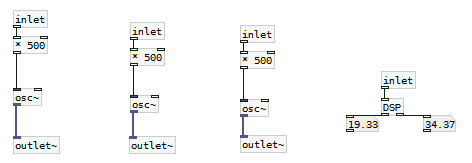
\includegraphics[width=1\textwidth]{Output}
\caption{The contents of \texttt{pd output}.}
\label{Fig:Output}
\end{figure}

\section{Image processing code}
When importing pictures into pure data a message called \texttt{open} is used. It takes a picture from a specific location and outputs it to \texttt{pix\_image} which is the object that is used for preparing an image for further use. \testtt{pix\_image} sends the image into the \texttt{pix\_draw} which draws the image directly onto the screen. After the images is drawn, it is then sent into the \texttt{pd imageprocessing} block which can be seen in Figure \ref{Fig:Imageprocessing}.

\begin{figure}
\centering
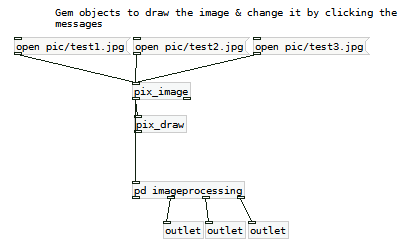
\includegraphics[width=1\textwidth]{Pdpictures}
\caption{The blocks that are responsible for image processing.}
\label{Fig:pdpicture}
\end{figure}

Inside the \texttt{pd imageprocessing} block a double nested for loop is implemented using an \texttt{expr} function in pure data. Through the use of three if statements, and taking advantage of the dataflow nature of Pure Data, the equivalent of a nested for loop is created which examines each pixel in the input image according to their x- and y-coordinate. The loop goes through 0 to 1. When it reaches 1 it adds 0.01 to another variable and resets to 0 to start over. When the second variable hits 1 it resets to 0 and the whole process starts over. The delay is placed so that the program doesn't preform a stack overflow when handling the if statements. 
As the if statements process data, a set of sliders have been placed to visualise the current pixel position, these sliders move in real time as the image is processed. The information contained in the pixel at position corresponding to these variables is then outputted to the \texttt{pix\_data} object, which takes a pixel position and a gem list and outputs the values of the RGB channels into three different numbers which is then outputted. 

\begin{figure}
\centering
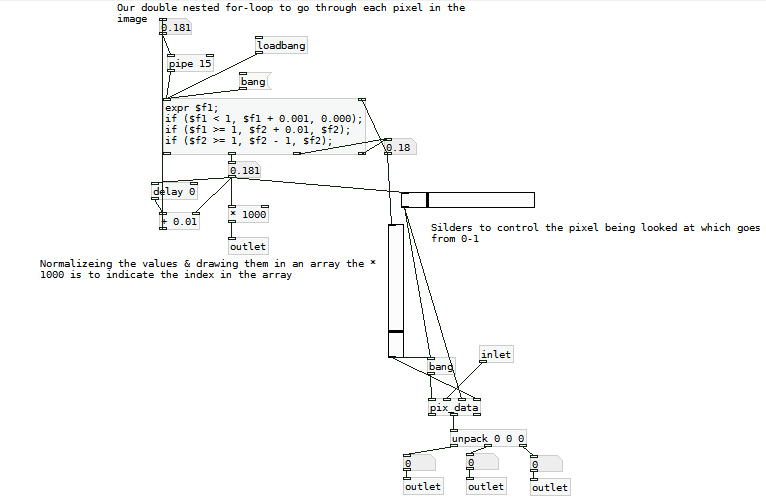
\includegraphics[width=1\textwidth]{Imageprocessing}
\caption{The contents of \texttt{pd imageprocessing}}
\label{Fig:Imageprocessing}
\end{figure}

\section{Filter code}

\begin{figure}
\centering
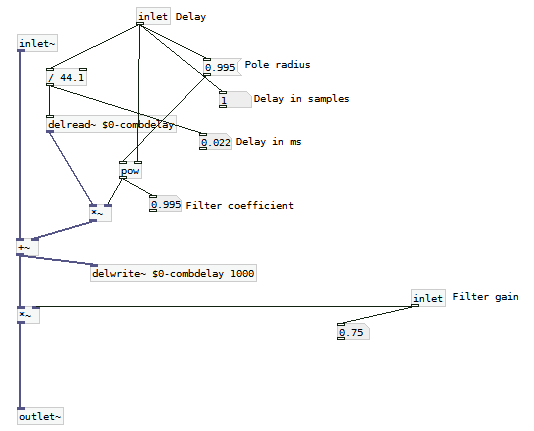
\includegraphics[width=1\textwidth]{Comb_filter}
\caption{The contents of the comb filter patch.}
\label{Fig:Comb_filter}
\end{figure}

\section{Arduino code}
For the Arduino a \texttt{pd arduino} patch has been made containing all the objects for the arduino part of the code. It takes a number and a list of 5 numbers as inputs. The first single number defines which serial port should be used to access the Arduino. The list of numbers defines which analogue inlets are open and which are closed. Each inlet is associated with a position in this list, and the number determines whether a given inlet is active (the number is 1) or inactive (the number is 0).

\begin{figure}
\centering
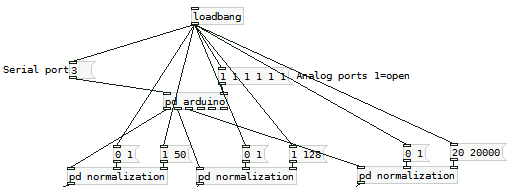
\includegraphics[width=1\textwidth]{Arduino_normalization}
\caption{The arduino blocks for inputs and outputs.}
\label{Fig:Arudino_normalization}
\end{figure}

After the inputs have been sent the serial port number is sent to a message \texttt{open \$1} which takes the number and places it at the \texttt{\$1} and then sends the message \texttt{open \$1} to the object \texttt{pduino/arduino}
which opens the serial port. The list of ones and zeroes is sent into an unpack taking six floats and unpacks them into six different messages, \texttt{analogIns 0 \$1}, \texttt{analogIns 1 \$1} and up to \texttt{analogIns 5 \$1}. It then sends all the messages into the \texttt{pduino/arduino} object.

The \texttt{pduino/arduino} object sends all of its data into its single outlet. This data contains information from all active in/outlets, digital or analog, as well as information about the Arduino device and how it is performing. The only piece of information the software needs is the data from the analog inlet. The \texttt{route} object is used to filter out all data that does not contain the "analog" label, and then another \texttt{route} object is used to sort the data according to the inlet it originates from. Finally a conversion is made so that the state of each inlet is represented with a floating point number between zero and one.


\begin{figure}
\centering
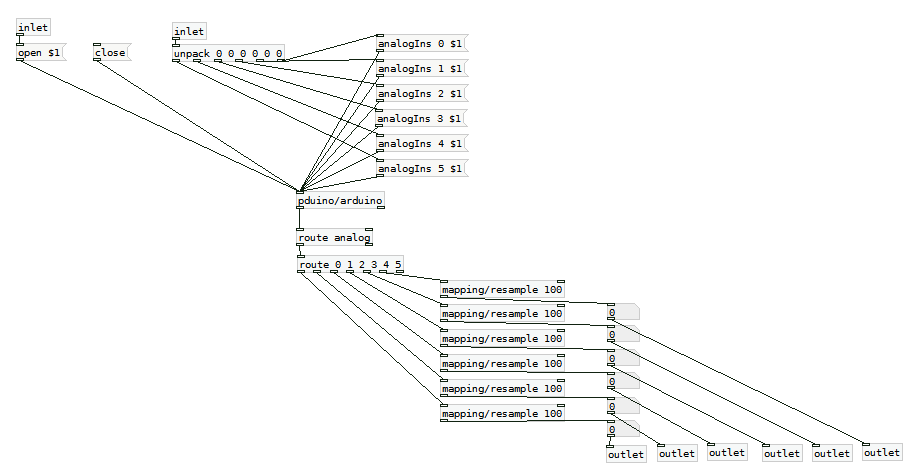
\includegraphics[width=1\textwidth]{Inside_arduino}
\caption{The contents of \texttt{pd arduino}.}
\label{Fig:Inside_arduino}
\end{figure}

The user defined parameters for the filters need numbers in various ranges. To achieve this, a patch called \texttt{pd normalization} is used to normalize the numbers from the analog inlets on the Arduino from the range of zero to one to a different range, depending on the filter. The object has three inlets; one for the raw data, one for the original data range, and one for the desired range. The patch then applies the equation $\frac{max'-min'}{max-min}\cdot (data-max)+max'$ where max' and min' make up the desired range, and max and min make up the original range. The result is then passed to the outlet.

\begin{figure}
\centering
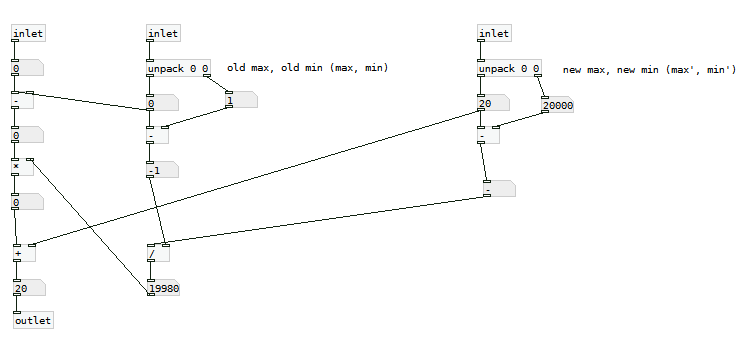
\includegraphics[width=1\textwidth]{Normalize}
\caption{The contents of \texttt{pd normalization}.}
\label{Fig:Normalize}
\end{figure}